%-------------------------------------------------------------------------------
\chapter{QCD corrections and uncertainties}
\label{sec:modelingCorr}
%-------------------------------------------------------------------------------

\todo{see also INT2, add that info here}

%%%%%

\section{PDF sets -- Filippo, Ludovica}

\textcolor{red}{PDF sets to be considered : CT18, CT18A, CT18Z; MSHT20; HERAPDF20; NNPDF31; NNPDF40 - all at NNLO. Any N3LO sets?}

\textcolor{red}{Plots and tables:
\begin{itemize}
\item rapidity distributions for W+, W-, Z, all PDFs
\item cross section tables for W+, W-, Z, all PDFs
\end{itemize}}

%%%%%

\section{Spin correlations -- Chen}

\textcolor{red}{Study reweighting accuracy and determine a systematic in the angular coefficients.}

\textcolor{red}{Reweighting accuracy : Ai reweighting at NLO with fine bins, NLO with wide bins, and NNLO with wide bins. Plots and tables:
\begin{itemize}
\item overlay the reweighted A0,...,A4 vs pT, in the three cases; compare with the reweighting targets
\item overlay the reweighted mT, pTl, pTnu in the three cases
\item compare with and without Ai interpolation
\item impact on mW (statistical-only fit)
\item study the effect of separately reweighting A0,...,A4 on the distributions and fits (cf. Fig.7 and Tab.7 of 2308.09417)
\item closure test : reweight Powheg in pT,y,Ai to dyturbo; compare the reweighted pTl and mT distributions with the resummed dyturbo distributions
\end{itemize}}

\textcolor{red}{Define strategy to define actual systematic. Some fraction of (NNLO-NLO)? Check approaches of LHCb, CMS.}

%%%%%

\section{Transverse momentum distribution with \textsc{Dyturbo} -- Filippo, Ludovica}

\subsection{Theoretical framework}

\subsection{Final-state distributions}

%%%%%

\section{Transverse momentum distribution using theory nuisance parameters -- Tanguy, Doriane, Filippo}

\textcolor{red}{Text, tables and plots:
\begin{itemize}
\item sketch of calculation, separation of singular, non-singular and hard terms, matching
\item illustration of matching procedure using an example PDF and $\sqrt{s}$ (eg CT18NNLO, 13 TeV)
\item illustration of TNP and NP variations
\item impact on final-state distributions : boson kinematics at generator level; pTl, mT, MET at detector level; one PDF in main body, others in appendix
\item NB : need 5, 13 and also 7 TeV
\end{itemize}}

\subsection{Matching resummed and fixed-order calculations}

\subsection{Theory nuisance parameters}

\subsection{Non-perturbative parameters}

\subsection{Final-state distributions}



%%%%%

\chapter{Application of QCD corrections -- Baris}

\section{Reweighting strategy}

\section{Closure tests}

%%%%%

\chapter{Electroweak corrections -- Xuewei, Shengpei, Maarten}

Finally, an evaluation of the remaining higher-order electroweak(EW) effects is presented.
The effects not addressed by the above studies include the interference
between initial- and final-state photon radiation, and genuine weak
corrections such as vertex and box diagrams.

Two programs are available for this study, which are briefly described below:
\begin{itemize}
  \item \textsc{Powheg} EW~[16,17]: a program combining
  $\mathcal{O}(\alpha_{\mathrm{S}})$ and $\mathcal{O}(\alpha)$ corrections to
  $W$ and $Z$ production; the \textsc{Pythia} parton shower for further initial-state
  parton and photon emissions; and \textsc{Photos} for further final-state photon
  emissions. The \textsc{Pythia} and \textsc{Photos} emissions are ``vetoed'', avoiding
  double counting with the emissions from the hard matrix element.

  \item \textsc{Winhac}~[18], based on \textsc{Sanc}~[15] for $W$ production described at
  $\mathcal{O}(\alpha)$, \textsc{Pythia} for initial-state parton and photon
  emissions, and two implementations of final-state radiation: \textsc{Photos} as
  above, and the \textsc{Yfs} formalism widely used at LEP.
\end{itemize}

Starting from a set of well-measured fundamental constants, electroweak
corrections can be computed in several schemes. Two schemes are used below:
\begin{itemize}
  \item the $\alpha_0$ scheme: the Born-level predictions are expressed in
  terms of the $W$- and $Z$-boson masses, $m_W$ and $m_Z$, and
  $\alpha_{\mathrm{QED}}(Q^2=0)\sim 1/137$;

  \item the $G_\mu$ scheme: the predictions are expressed in terms of $m_W$,
  $m_Z$, and $G_\mu$, implying a tree-level QED effective coupling constant
  given by
  \begin{equation}
    \alpha_{G_\mu}
    = \frac{\sqrt{2}\,G_\mu \sin^2\theta_W\,m_W^2}{\pi}
    \sim \frac{1}{133}.
  \end{equation}
\end{itemize}

The latter is generally considered more accurate, as the initial value of the
electromagnetic coupling constant already accounts for part of its evolution
between $\alpha(Q^2=0)\sim 1/137$ and $\alpha(Q^2=m_Z^2)\sim 1/128$, therefore
incorporating a subset of corrections formally beyond
$\mathcal{O}(\alpha)$.

In the following sections, we present a study of the decomposition of the EW
corrections using \textsc{Winhac}, a comparison of the \textsc{Powheg} EW and \textsc{Winhac}
predictions, and finally an evaluation of the impact of these corrections on
the measurement. All distributions are shown at generator level and without
any cuts, to maximize the sample statistics and the size of the observed
effects.



\section{Decomposition of EW corrections}

\textsc{Winhac} provides handles to study separately the effect of FSR, full QED
(i.e.\ FSR, ISR, and ISR/FSR interference), and full
$\mathcal{O}(\alpha)$ corrections (i.e.\ QED plus the remaining weak
corrections). Figure~11 illustrates the various contributions for the
$m_{\ell,\nu}$, $m_T$, $p_T^\ell$, and $p_T^\nu$ distributions. The QCD
parton shower is switched off, i.e.\ $p_T^W\sim 0$; the
$\mathcal{O}(\alpha)$ corrections are computed in the $G_\mu$ scheme.
Comparison to the Born prediction (left column) shows, as expected, that the
FSR correction dominates the full correction, representing about 99\% of the
overall effect. The effect is largest on the $m_{\ell,\nu}$ distribution.

Removing the Born prediction (Figure~11, right column), and comparing the
remaining predictions to the FSR distributions obtained using \textsc{Yfs}, shows
that:
\begin{itemize}
  \item the \textsc{Yfs} and \textsc{Photos} FSR predictions match perfectly, in agreement
  with the small uncertainty on this component discussed in Section~2.3;
  \item non-FSR QED effects represent about two thirds of the total remaining
  corrections; pure weak effects are sub-leading;
  \item the corrections are largest in the $p_T^\ell$ distribution and
  minimal in the $p_T^\nu$ distribution. The $m_T$ distribution, built from
  the previous two, is in between.
\end{itemize}

The study is repeated in Figure~12, with the QCD parton shower switched on. As
expected, the $m_{\ell,\nu}$ and $m_T$ predictions are unaffected, as the QCD
emissions typically have low $p_T$ compared to the invariant mass of the
final state, and hardly limit the phase space available for the hard process.
In contrast, the effects on the $p_T^\ell$ and $p_T^\nu$ distributions are
washed out due to the non-trivial $p_T^W$ distribution.

The differences between the FSR- and EW-corrected distributions in the
presence of the parton shower, i.e.\ the right columns in Figure~12, are
relevant to quantify the effects missing in the MC samples. The relative
differences are at the level of 0.1\% or below, with a smooth behaviour around
the Jacobian peaks.

\subsection{FSR}
FSR in nominal sample is handled by PHOTOS.
Figure \ref{} shows the kinematic distributions with and without FSR corrections, illustrating the overall impact of FSR. The muon kinematics are shown at the bare level, while the electron kinematics are presented at the dressed level, where the bare electron is combined with all photons within $\Delta R < 0.1$, roughly mimicking the photon collections in calorimeters. The height of the invariant mass peak decreases by a few percent accompanied by a slight increase in the tails at lower masses. A similar effect is observed in the Jacobian peak for the lepton transverse momentum distribution. FSR acts as the dominant effect among the electroweak modifications.
The uncertainty from the FSR modeling is estimated through a comparison between FSR simulations conducted by PHOTOS and those employed in the Yennie–Frautschi– Suura (YFS) scheme \cite{} widely used at LEP that separates the infrared divergences into multiplicative factors.


\subsection{QED and $\mathcal{O}(\alpha)$}
In the context of EW radiative corrections, the notation $\mathcal{O}(\alpha)$ denotes the first-order (one-loop) contribution in the perturbative expansion with respect to the fine-structure constant $\alpha \equiv e^2/(4\pi) \approx 1/137$. The theoretical prediction for a generic observable can be organised as
\begin{equation}
    \sigma = \sigma_{\mathrm{LO}} \Bigl( 1 + \delta_{\mathrm{EW}} + \delta_{\mathrm{QCD}} + \cdots \Bigr),
    \label{eq:perturbative_expansion}
\end{equation}
where $\delta_{\mathrm{EW}} \propto \alpha$ corresponds to the full set of Feynman diagrams containing one internal electroweak gauge boson ($\gamma$, $W^{\pm}$, $Z^{0}$) or Higgs loop. Concretely, $\mathcal{O}(\alpha)$ EW corrections encompass virtual corrections from $\gamma$, $W^{\pm}$, and $Z^{0}$ propagators inside loops, real photon radiation from external charged legs (initial- and final-state radiation, ISR/FSR), and sub-leading Higgs-loop contributions. The Feynman diagrams of these processes are as below:

\begin{figure}[h!]
    \centering
    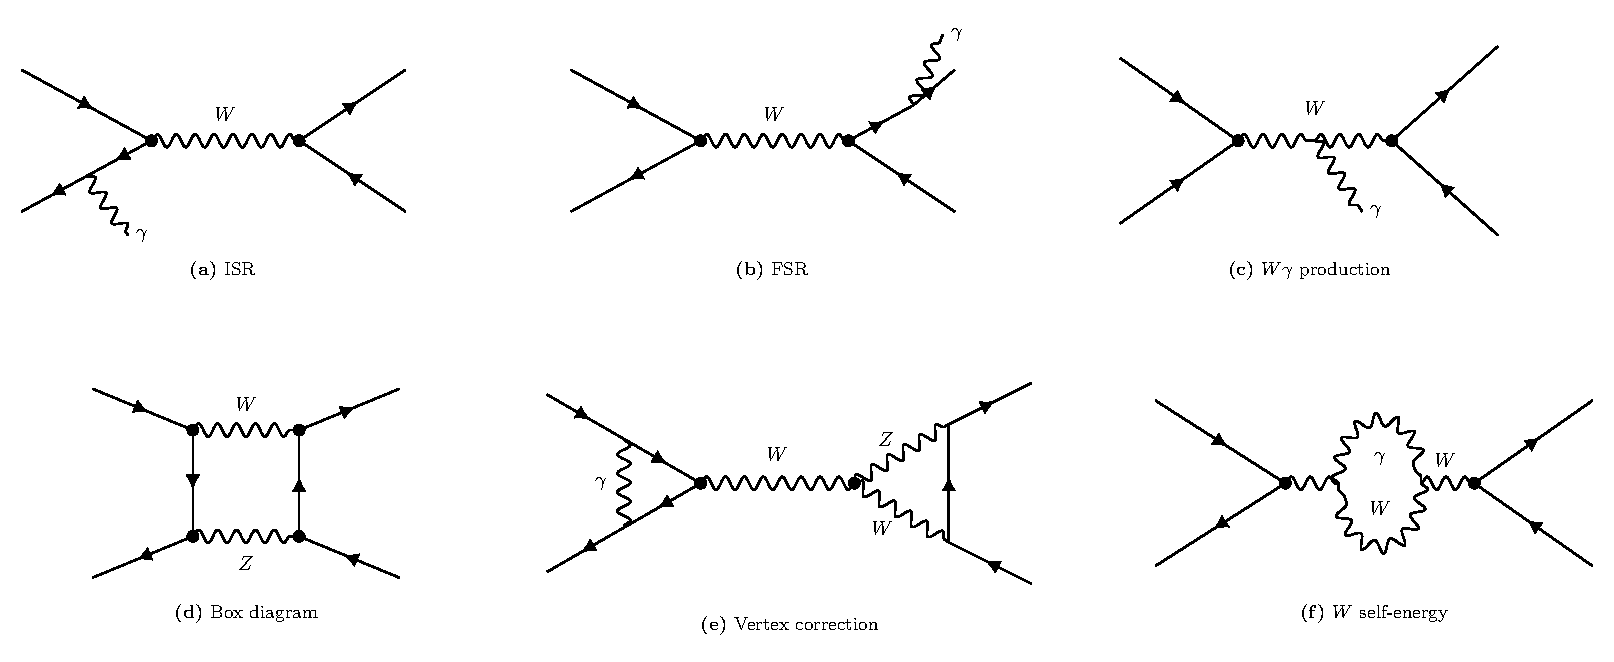
\includegraphics[width=1.0\textwidth]{figures/electroweak/EW_correction_feynman_diagrams.pdf}
    \caption{Representative Feynman diagrams of $\mathcal{O}(\alpha)$ EW corrections in $pp\to W^{\pm}\to\ell^{\pm}\nu_{\ell}$ processes.}
    \label{fig:ew_diagrams}
\end{figure}
    
The full set of $\mathcal{O}(\alpha)$ EW corrections to hard processes
with an on-shell $W$ boson in the final state, such as $pp\to W^{\pm}\to\ell^{\pm}\nu_{\ell}$,
can be organised along two complementary axes.

\paragraph{Real vs.\ virtual corrections.}
\textit{Virtual corrections} consist of all one-loop Feynman diagrams contributing
to the Born-level $2\to 2$ (or $2\to 1$) amplitude.
They include vertex corrections to the $q\bar{q}'W$ and $W\ell\nu$ couplings,
fermion and gauge-boson self-energies ($\Sigma_{WW}$, $\Sigma_{ZZ}$, $\Sigma_{\gamma\gamma}$,
$\Sigma_{\gamma Z}$, and the corresponding fermion-loop insertions), and box diagrams
involving $\gamma$, $W^{\pm}$, and $Z^{0}$ exchange.
Virtual amplitudes are complex-valued, contain both ultraviolet (UV) and infrared (IR)
divergences, and do not alter the multiplicity of the final state.

\textit{Real corrections} consist of tree-level diagrams with an additional photon
radiated from any electrically charged external leg --- initial-state radiation (ISR)
off the incoming quarks and final-state radiation (FSR) off the outgoing charged lepton and
the $W$ boson itself, together with their interference terms.
These amplitudes are real-valued (no loop integrals), UV-finite, but
develop IR and collinear singularities when the photon becomes soft or collinear
to a radiating fermion.

In isolation, virtual photon loop diagrams and real photon emission diagrams both contain soft infrared divergences: the former diverge when the energy of the loop photon tends to zero, and the latter diverge when the energy of the emitted photon tends to zero. The Bloch--Nordsieck(KLN) theorem guarantees that these two divergences cancel, at every point in phase space, exactly once the contributions are added together. This cancellation holds because a detector cannot distinguish a bare charged particle from a charged particle accompanied by an arbitrarily soft photon; therefore, the physically observable cross section must include both types of contributions summed over all such indistinguishable configurations.
Collinear singularities, which appear as logarithms of light-fermion masses,
$\ln(Q^{2}/m_{\ell}^{2})$, can be treated either by retaining finite fermion masses
(mass regularisation), by dimensional regularisation with $\overline{\mathrm{MS}}$
subtraction, or by absorbing them into non-perturbative QED fragmentation functions.

\paragraph{Photonic(QED) vs.\ genuinely weak corrections.}
A further physically motivated decomposition separates the full $\mathcal{O}(\alpha)$
result into a \textit{photonic} (QED-like) part and a \textit{genuinely weak} part.

The photonic subset collects all diagrams that contain at least one internal photon
propagator: virtual photon loops (vertex, self-energy, and box topologies),
the $\gamma$--$Z$ mixing self-energy $\Sigma_{\gamma Z}$, and the entire
tree-level bremsstrahlung contribution $\ell^{\pm}\nu_{\ell}\gamma$.
This subset carries the full IR structure of the EW corrections:
soft and collinear divergences appear in both the virtual and the real components
and cancel only in their sum.

The genuinely weak part comprises all remaining one-loop diagrams that involve
only massive gauge bosons ($W^{\pm},Z^{0}$) and the Higgs boson in the internal
lines, i.e.\ $W/Z$ self-energies, $W/Z$ vertex corrections, and $W/Z$ box diagrams
(with negligible Higgs contributions). Because $M_W$ and $M_Z$ provide a natural
infrared cut-off, the genuinely weak subset is free of soft and collinear
divergences --- it is IR-finite on its own, without invoking real-emission
cancellations. Its dominant phenomenological signature at high energies is the
electroweak Sudakov enhancement, $\frac{\alpha}{\pi}\ln^{2}(Q^{2}/M_{W}^{2})$,
which grows with the partonic centre-of-mass energy.

\paragraph{Gauge invariance of the decomposition.}
While the \emph{complete} $\mathcal{O}(\alpha)$ correction (virtual $+$ real
$+$ counterterms, properly renormalised) is a gauge-invariant physical observable,
the \emph{splitting} into photonic and genuinely weak components is not gauge-invariant
on its own.

The assignment of a given Feynman diagram to the photonic or the weak
category depends explicitly on the choice of the gauge-fixing parameter.
In the standard 't~Hooft--Feynman gauge ($\xi=1$), the decomposition relies
on the particle content of the internal propagator: a diagram is classified as
photonic if it contains a photon propagator and as genuinely weak otherwise.
A change of gauge may reshuffle contributions between the two subsets, so that
the numerical values of the two parts are individually gauge-dependent;
only their sum is physically meaningful.

\subsection{Comparison of NLO EW corrections in \textsc{Winhac} and \textsc{Renesance}}
There is another MC generator, \textsc{Renesance}, which is based on the same \textsc{SANC} framework as \textsc{Winhac}. These two generators deal with EW corrections in different ways, and the comparison of their predictions provides a useful cross-check of the implementation.

At the parton level they share a common theoretical ingredient: the EW one-loop virtual corrections are evaluated with the same \textsc{SANC} library developed at JINR, which provides the self-energy, vertex, and box contributions together with the counterterms required in the on-shell renormalisation scheme. 

The difference lies in how the real photon radiation is organised. \textsc{ReneSANCe} remains strictly at fixed next-to-leading order (NLO) in the EW coupling: the cross section is decomposed into a Born term, a virtual-plus-soft term, and a hard single-photon term, without resumming higher-order soft-photon logarithms. \textsc{Winhac}, by contrast, adds the complete Yennie--Frautschi--Suura (YFS) exclusive exponentiation on top of the \textsc{SANC} virtual corrections. This means that multiple photons can be emitted in each event, and the leading soft-photon logarithms are resummed to all orders in $\alpha$.

The YFS exclusive exponentiation scheme provides an infrared-safe prescription for resumming multiple soft-photon emission to all orders in perturbation theory. Its starting point is the factorisation of the radiation cross section into a soft-photon distribution multiplied by a hard process whose infrared singularities have been subtracted. For a charged-particle line connecting an initial quark $i$ to a final lepton $f$, the universal YFS form factor $Y$ collects the leading logarithms from the soft region:
\begin{equation}
    Y(p_i,p_f) = 2\alpha\,\Re\!
    \int\!\frac{d^4 k}{(2\pi)^3}\,
    \frac{\delta_+(k^2)}{k^0}\,
    \frac{p_i\cdot p_f}{(p_i\cdot k)(p_f\cdot k)}\,
    \Theta(k^0 - k_{\max})\,,
    \label{eq:yfs_form_factor}
\end{equation}
where the cut-off $k_{\max}$ separates the soft-photon phase space that is resummed from the hard-photon remainder that is treated at fixed order.

Physically, the YFS exclusive exponentiation scheme separates the radiation process into
two distinct regimes: \emph{many soft photons} and \emph{few hard photons}.
Soft photons, with energies $k^0 \ll k_{\max}$, can be emitted an arbitrary number of
times by the charged external legs. Although each individual soft photon carries very
little energy, their collective emission probability is not negligible because there is
no upper limit on how many of them can be radiated. Computing this regime order by order
in fixed perturbation theory would require summing over an increasing number of
soft-photon emission diagrams at every higher order, each plagued by infrared
divergences in the low-energy limit.

The YFS prescription reorganises the radiative cross section as a product of a
\emph{soft-photon distribution function} and a \emph{hard process} from which infrared
singularities have been subtracted. The soft-photon distribution resums all multi-photon
emissions with energies below $k_{\max}$, while the hard process contains only photons
above $k_{\max}$ and can be computed reliably with ordinary fixed-order perturbation
theory. The universal form factor $Y(p_i,p_f)$ accumulates the leading logarithms from
the soft region, exponentiating them into an overall factor $\exp[Y(p_i,p_f)]$.
Because any realistic detector has finite energy resolution, it cannot distinguish
``no soft-photon emission'' from ``emission of arbitrarily soft photons''. The YFS
exponentiation includes the full tower of such indistinguishable multi-photon states,
thereby guaranteeing infrared-safe predictions for physical observables.

The exponentiation of $Y$ follows from the independence of soft-photon emissions
in the eikonal limit. For a charged line connecting $p_i$ to $p_f$, the amplitude
for radiating a single soft photon factorises into the eikonal current
$J^\mu(k) = p_f^\mu/(p_f\!\cdot\!k) - p_i^\mu/(p_i\!\cdot\!k)$, and multiple
soft photons decouple: the $n$-photon soft amplitude reduces to the product of
$n$ such independent factors. Summing the Poisson-distributed soft-photon
multiplicities to all orders yields
\begin{equation}
    \sum_{n=0}^{\infty} \frac{1}{n!} \prod_{j=1}^{n} \int_{k_{\min}}^{k_{\max}}
    \frac{d^{3}k_{j}}{2k_{j}^{0}} \,
    \tilde{S}(k_{j})
    \;=\; \exp\!\left[\, \int_{k_{\min}}^{k_{\max}}
    \frac{d^{3}k}{2k^{0}} \, \tilde{S}(k) \right]
    \;=\; \exp\bigl[\,Y(p_i,p_f)\bigr]\,,
    \label{eq:yfs_exponentiation}
\end{equation}
where the eikonal factor
$\tilde{S}(k) \propto p_i\!\cdot\!p_f / [(p_i\!\cdot\!k)(p_f\!\cdot\!k)]$
recovers the integrand of Eq.~\eqref{eq:yfs_form_factor}, and the band
$k_{\min}\lesssim k^0\lesssim k_{\max}$ delimits the soft-photon phase space
that is resummed. The Poisson structure of the sum over soft multiplicities
guarantees that the infrared singularities cancel between virtual and real
contributions once the detector resolution $k_{\min}$ is taken to zero,
leaving a finite exponent that depends only on the soft--hard separation
scale $k_{\max}$.

In the exclusive formulation, the event weight is written as the product of an exponential factor and a finite remainder,
\begin{equation}
    w = \exp\bigl[Y\bigr]\;\prod_{j=1}^{n}\,\tilde{S}(k_j)\;
    \Bigl( 1 + \delta^{(1)}_{\mathrm{hard}}\Bigr)\,,
    \label{eq:yfs_weight}
\end{equation}
where $\tilde{S}(k_j)$ is the normalised single-photon eikonal distribution and $\delta^{(1)}_{\mathrm{hard}}$ contains the first-order hard-photon correction evaluated from the exact matrix element. The Monte Carlo generates the photon multiplicity $n$ from a Poisson-like distribution governed by $\exp[Y]$, and samples each photon momentum from $\tilde{S}(k_j)$. The real-emission singularities of $\delta^{(1)}_{\mathrm{hard}}$ exactly cancel those implicitly contained in $\exp[Y]$, so that the fully differential cross section is infrared finite. This procedure goes beyond fixed-order NLO because it includes the emission of two, three, or more soft/collinear photons with the correct leading-logarithmic weight, while preserving the exact first-order hard-photon matrix element.

\textsc{Winhac} simulates the full partonic process $q\bar{q}'\to W\to \ell\nu_\ell$ together with QED initial-state radiation (ISR), final-state radiation (FSR), and the electroweak one-loop corrections. The event generation proceeds in two stages. First, the hard-scattering kinematics are constructed including the exact first-order EW virtual corrections from \textsc{SANC}. Second, the YFS exponentiation module generates the photon ensemble: photons are emitted in the rest frame of the decaying $W$ and then boosted back to the laboratory frame, allowing a natural separation between the soft/collinear regime and the hard-photon region. The resulting event record contains the charged fermions and an arbitrary number of real photons, weighted according to Eq.~\eqref{eq:yfs_weight}.

When \textsc{Winhac} is interfaced to a general-purpose parton shower such as \textsc{Pythia}, the two programs must be coordinated to avoid counting the same QED initial-state radiation twice. The difficulty arises because \textsc{Winhac}, through its YFS exponentiation, already resums soft and collinear ISR logarithms to all orders and generates an explicit ensemble of photons, while \textsc{Pythia} simultaneously performs both QCD and QED initial-state showers on the incoming partons.

The solution adopted in \textsc{Winhac} is to treat the ISR at the weight level, by controlling how much of the QED initial-state contribution is absorbed into the YFS exponential factor. Three physically distinct prescriptions are available. In the first, the Marciano--Sirlin (MS) scheme, the YFS exponentiation covers only final-state radiation and the initial--final interference; the ISR is kept at fixed order and is left entirely to \textsc{Pythia}. In the second, the YFS-like scheme, a YFS-motivated form factor is used for the ISR correction at fixed order. In the third, the dipole-subtraction (DSM) scheme---the recommended choice---the ISR contribution is fully included in the YFS exponential factor, resumming its leading logarithms to all orders, while a dipole subtraction is applied to the first-order hard-photon matrix element. This removes the leading-logarithmic ISR piece that would otherwise be generated again by \textsc{Pythia}, retaining only the process-dependent, non-logarithmic remainder of the exact $\mathcal{O}(\alpha)$ matrix element. The YFS-generated photons, together with the decay leptons, are passed to \textsc{Pythia} as a set of final-state particles, upon which \textsc{Pythia} then builds its QCD+QED shower and performs hadronisation. (\textcolor{red}{need to check and verify later}) 

\textsc{ReneSANCe}, different from Winhac, generates the charged-current Drell--Yan process events by calculating fixed-order NLO EW partonic cross section. The differential distribution is split into four independent contributions:
\begin{equation}
    d\sigma = d\sigma_{\mathrm{Born}}
    + d\sigma_{\mathrm{Virt}}
    + d\sigma_{\mathrm{Hard}}
    + d\sigma_{\mathrm{Brdq}}\,,
    \label{eq:renesance_splitting}
\end{equation}
where $d\sigma_{\mathrm{Born}}$ is the lowest-order cross section, $d\sigma_{\mathrm{Virt}}$ combines the one-loop virtual corrections with the soft-photon emission up to a small cut-off $E_\gamma^{\min}$, $d\sigma_{\mathrm{Hard}}$ contains the emission of a single photon with energy above $E_\gamma^{\min}$, and $d\sigma_{\mathrm{Brdq}}$ is the quark-mass subtraction term that removes the initial-state collinear singularities regularised by finite light-quark masses.

The virtual corrections are obtained from the \textsc{SANC} library, while the real-photon matrix elements are evaluated with the complete helicity amplitudes for $q\bar{q}'\to W\to \ell\nu_\ell\gamma$. Each term in Eq.~\eqref{eq:renesance_splitting} is integrated separately with an adaptive Monte Carlo and combined at the histogramming level. Since only one hard photon is ever present in the final state, the program is strictly an NLO EW generator: it does not resum higher-order soft-photon logarithms and it does not attempt to match to a parton shower. This makes \textsc{ReneSANCe} particularly useful as a reference for the total NLO EW cross section and for differential distributions in observables where higher-order photon emission is expected to be small.

In summary, \textsc{Winhac} and \textsc{ReneSANCe} differ mainly in the treatment of real photon radiation, while their one-loop virtual electroweak corrections are effectively identical because both rely on the \textsc{SANC} library. \textsc{ReneSANCe} performs a strict fixed-order NLO EW calculation: the cross section is decomposed into Born, virtual+soft, hard single-photon, and quark-mass subtraction terms, and each event contains at most one hard photon. \textsc{Winhac}, on the other hand, implements the YFS exclusive exponentiation, which generates multiple soft and collinear photons and resums their leading logarithms to all orders. The price of this resummation is a more involved matching to external parton-shower programs such as \textsc{Pythia}, for which \textsc{Winhac} provides several subtraction schemes to avoid double counting of the initial-state QED radiation.

\section{Scheme dependence and impact on the \texorpdfstring{$m_W$}{mW}
measurement}

To evaluate the impact on the $m_W$ measurement, pseudo-data are generated
including full $\mathcal{O}(\alpha)$ corrections, and templates are generated
for different values of $m_W$ and including only FSR corrections. The
$W$-boson mass is then fitted as in Section~2.5, and the difference between
the fitted and injected values is taken as the systematic uncertainty related
to this effect. This exercise is repeated for both schemes, with the parton
shower switched on.

The results are summarized in Table~\ref{tab:ew-beyond-fsr}. The effects are generally found to be
larger for $G_\mu$, with typically 3.5~MeV for the $p_T^\ell$
distributions, 2.5~MeV for $m_T$, and 0.6~MeV for $p_T^\nu$. The statistical
accuracy of these estimates is about 0.2~MeV. As these effects are absent from
the full simulation samples, the full size of the effect found for $G_\mu$ is
taken as the uncertainty estimate.

\begin{table}[htbp]
  \centering
  \caption{Systematic effect on the $m_W$ measurement (in MeV) from EW
  corrections beyond FSR, in the $G_\mu$ and $\alpha_0$ schemes.}
  \label{tab:ew-beyond-fsr}
  \begin{tabular}{lccccc}
    \toprule
    Scheme & $p_T^e$ & $m_T^{e\nu}$ & $p_T^\nu$ & $p_T^\mu$
           & $m_T^{\mu\nu}$ \\
    \midrule
    $G_\mu$    & 3 & 3 & 3       & 3 & 3 \\
    $\alpha_0$ & 3& 3 & $3$   & 3 & 3 \\
    \bottomrule
  \end{tabular}
\end{table}


\textcolor{red}{Text, tables and plots (all inclusive in eta -- categories will be used for the fit):
\begin{itemize}
\item generator-level variations
\item migration matrices
\item impact at detector level
\end{itemize}}

\subsection{Input Parameter Schemes(IPS)}
In electroweak (EW) precision calculations, an input parameter scheme (IPS) specifies which measured quantities are used as independent inputs to define the renormalized EW theory. At the Lagrangian level, the EW interactions may be described in terms of parameters such as the gauge couplings $g$ and $g'$ and the Higgs vacuum expectation value $v$. In phenomenological calculations, however, these parameters are usually traded for experimentally measured observables, such as
$$
\alpha,\qquad G_\mu,\qquad M_W,\qquad M_Z,
$$
from which the derived quantities entering the matrix elements are obtained. 
Thus, choosing IPS amounts to deciding which quantities are fixed directly from experiment and which ones are derived through EW relations.

The role of an IPS becomes particularly important once radiative corrections are included. The relation between the precisely measured muon-decay constant $G_\mu$ and the EW parameters can be schematically written as
$$
\frac{G_\mu}{\sqrt{2}}
=
\frac{\pi\alpha}{2s_W^2 M_W^2}
\frac{1}{1-\Delta r},
$$
where $\Delta r$ represents radiative corrections, including contributions from the running of the electromagnetic coupling, weak-boson self-energies, and top-quark-mass dependent corrections. Different IPS choices correspond to absorbing different parts of these universal corrections into the lowest-order coupling. In an all-order calculation this is only a reparametrization, and all schemes would give the same physical prediction. At finite perturbative order, however, the residual dependence on the IPS reflects missing higher-order EW corrections.

Three commonly used schemes are the $\alpha(0)$, $G_\mu$, and $\alpha(M_Z^2)$ schemes. In the $\alpha(0)$ scheme, the electromagnetic coupling is defined in the Thomson limit,
$$
\alpha(0) \simeq \frac{1}{137},
$$
and the lowest-order coupling is obtained from
$$
e^2 = 4\pi\alpha(0),
\qquad
g^2 = \frac{4\pi\alpha(0)}{s_W^2}.
$$
This scheme is natural for real photon radiation, since photons emitted in final-state QED radiation couple at low momentum transfer. However, for hard EW processes at the scale of the weak boson masses, the use of $\alpha(0)$ leaves large light-fermion vacuum-polarization effects, usually denoted by $\Delta\alpha$, in the explicit higher-order corrections. This can lead to relatively large finite-order EW corrections.

In the $G_\mu$ scheme, the Fermi constant measured in muon decay is used as an input together with $M_W$ and $M_Z$. The effective electromagnetic coupling is defined as
$$
\alpha_{G_\mu}
=
\frac{\sqrt{2}G_\mu M_W^2 s_W^2}{\pi},
$$
or equivalently,
$$
g^2 = 4\sqrt{2}G_\mu M_W^2.
$$
This definition absorbs important universal corrections contained in $\Delta r$, including the running of $\alpha$ from low energies to the EW scale and leading corrections associated with the $\rho$ parameter. As a result, the $G_\mu$ scheme usually gives smaller explicit EW corrections and better perturbative stability for charged-current Drell--Yan production. For this reason, it is commonly used as the nominal scheme for modelling $W$ and $Z$ boson production at hadron colliders.

The $\alpha(M_Z^2)$ scheme instead uses the electromagnetic coupling evaluated at the $Z$-boson mass scale. In this case,
$$
e^2 = 4\pi\alpha(M_Z^2),
$$
where $\alpha(M_Z^2)$ already includes the dominant running of the electromagnetic coupling from $q^2=0$ to the EW scale. This reduces the large $\Delta\alpha$ contribution present in the $\alpha(0)$ scheme. However, unlike the $G_\mu$ scheme, it does not absorb the full set of universal weak corrections associated with muon decay. It therefore provides an intermediate choice between the $\alpha(0)$ and $G_\mu$ schemes and is useful for assessing the scheme dependence of the EW prediction.

For a direct measurement of the $W$-boson mass, the choice of IPS affects the theoretical templates used to extract $M_W$. The Born-level amplitude for charged-current Drell--Yan production,
$$
q\bar{q}' \to W^\pm \to \ell^\pm\nu,
$$
is proportional to the weak coupling, schematically
$$
\mathcal{M}_{\text{Born}} \propto g^2,
$$
so different definitions of $g$ lead to different normalizations and different allocations of radiative effects between the lowest-order prediction and the explicit EW corrections. Although most of the scheme dependence appears as an overall normalization effect, small shape differences can also arise in observables used in the $M_W$ fit, such as the charged-lepton transverse momentum, the missing transverse momentum, and the transverse mass. Therefore, comparisons between the $\alpha(0)$, $G_\mu$, and $\alpha(M_Z^2)$ schemes are commonly used as a systematic cross-check of EW modelling, with the scheme variations interpreted as part of the uncertainty due to missing higher-order EW corrections.

\section{Detector-level EW corrections}

\section{Estimate EW uncertainty}
\subsection{Template fit}



\begin{figure}[h!]
    \centering
    \begin{minipage}[b]{0.48\textwidth}
        \centering
        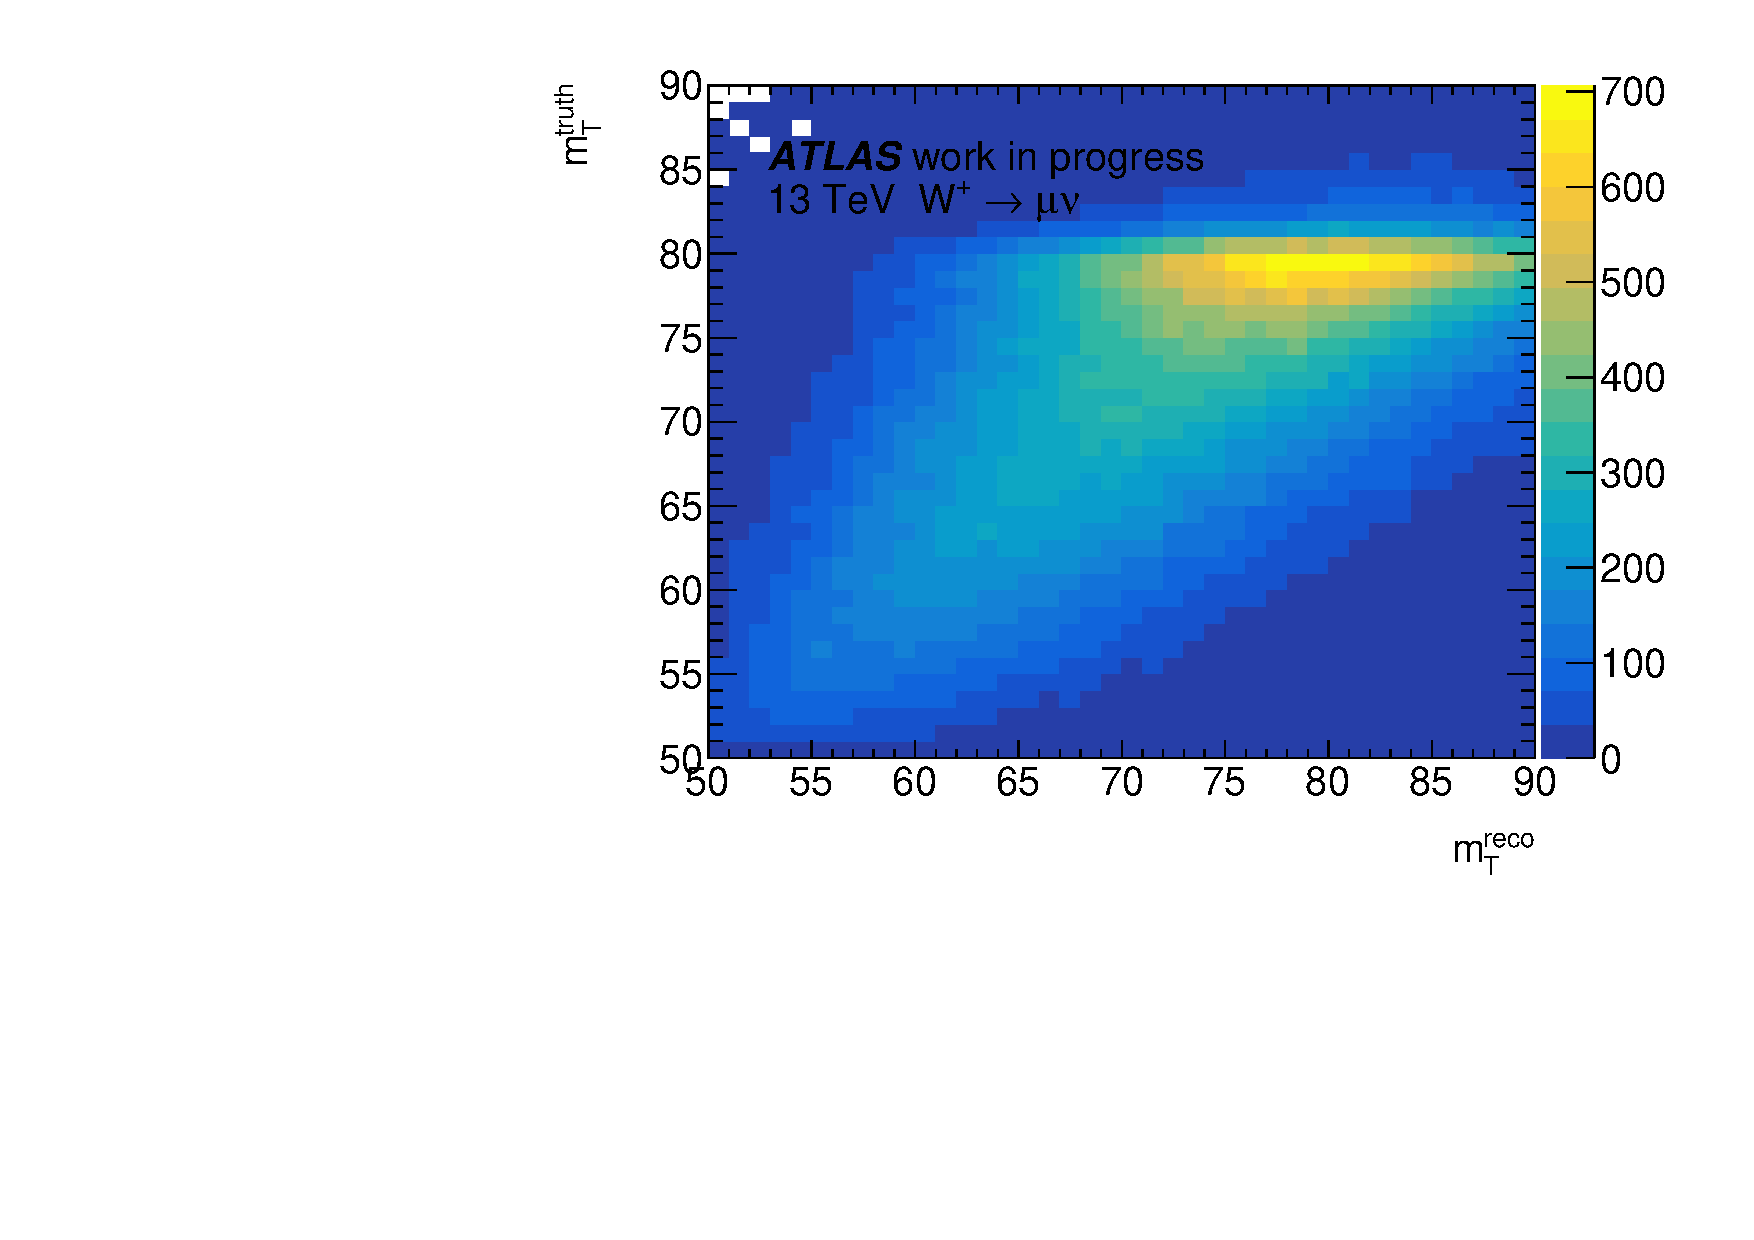
\includegraphics[width=\textwidth]{figures/electroweak/mig_13tev_Wplusmunu_mt.pdf}
    \end{minipage}
    \hfill
    \begin{minipage}[b]{0.48\textwidth}
        \centering
        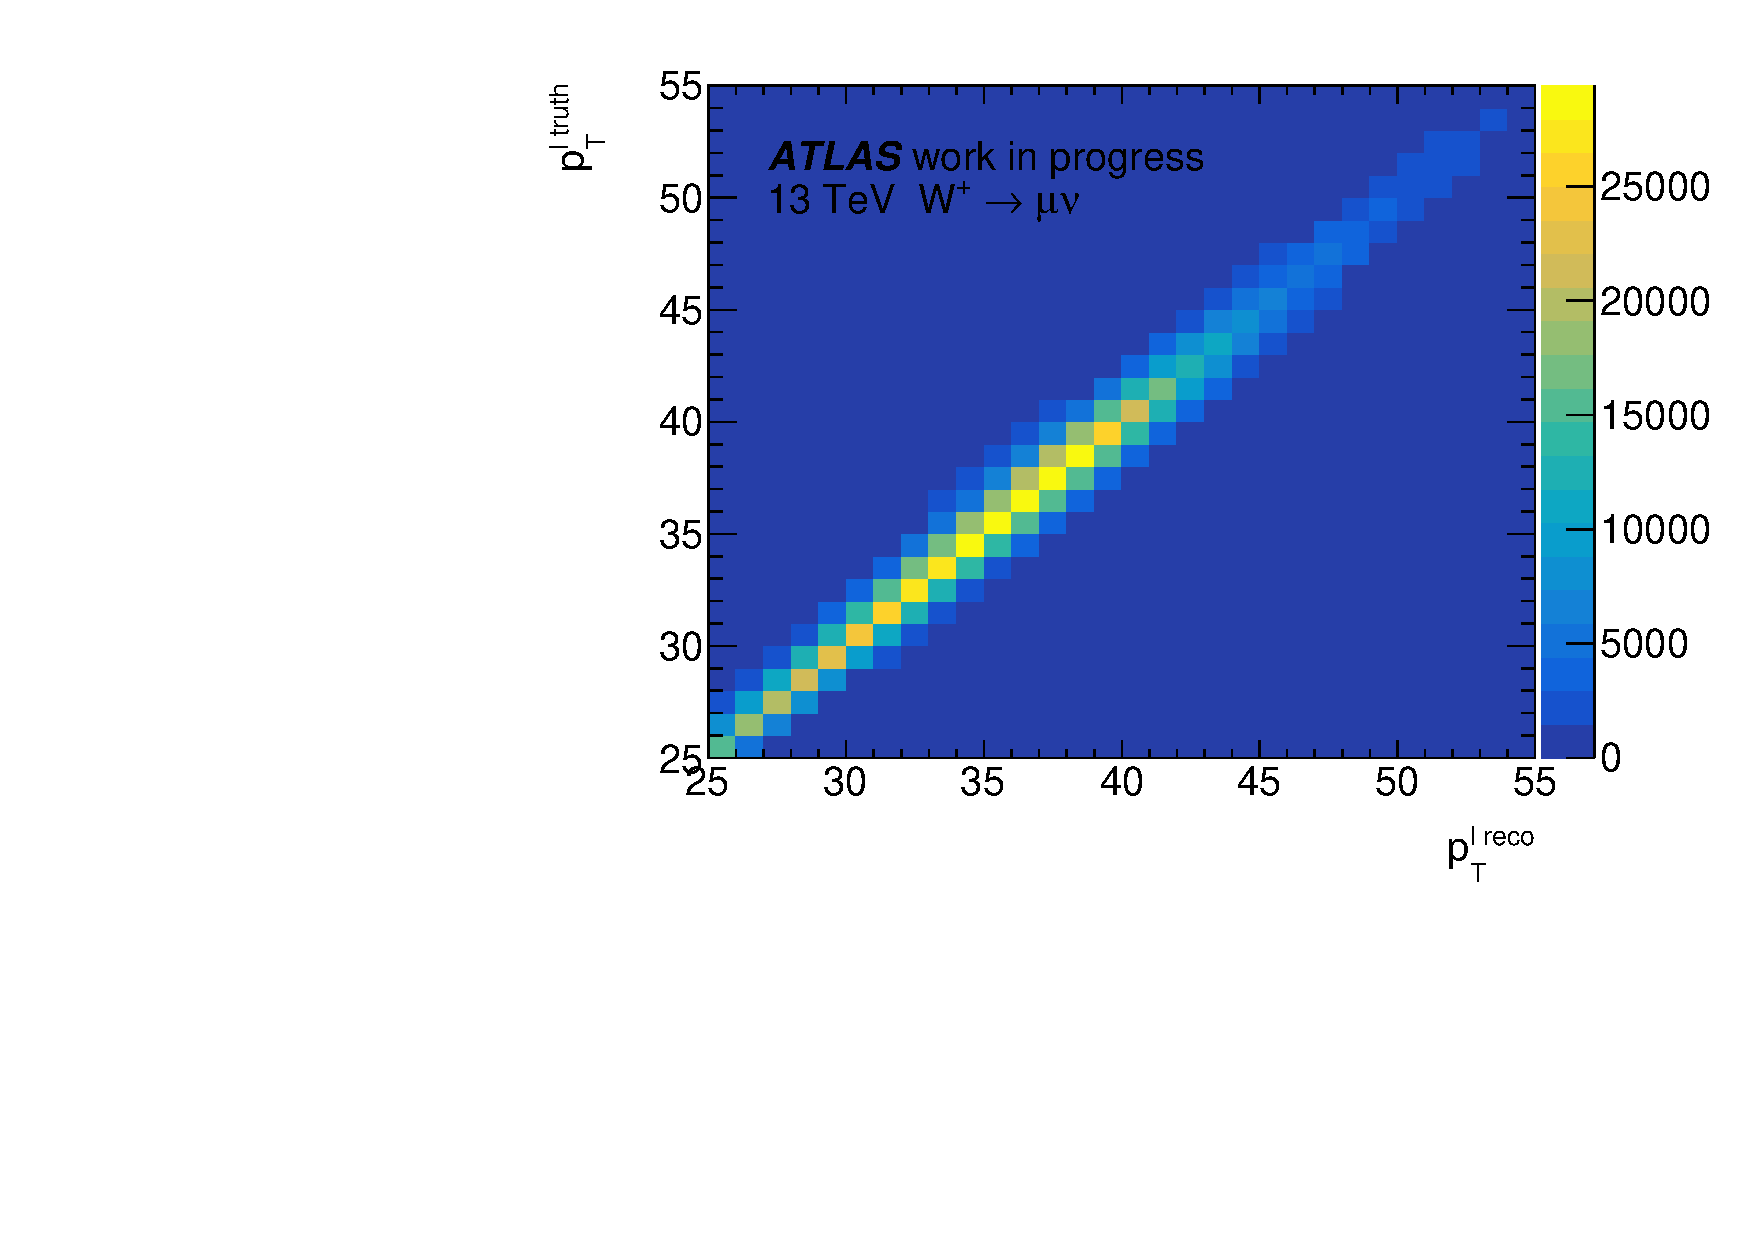
\includegraphics[width=\textwidth]{figures/electroweak/mig_13tev_Wplusmunu_LpT.pdf}
    \end{minipage}
      \caption{Migration matrix for 13 TeV wpmn lepton mt and lpt distribution.}
    \label{fig:mig13_lpt}
\end{figure}

\begin{figure}[h!]
    \centering
    \begin{minipage}[b]{0.48\textwidth}
        \centering
        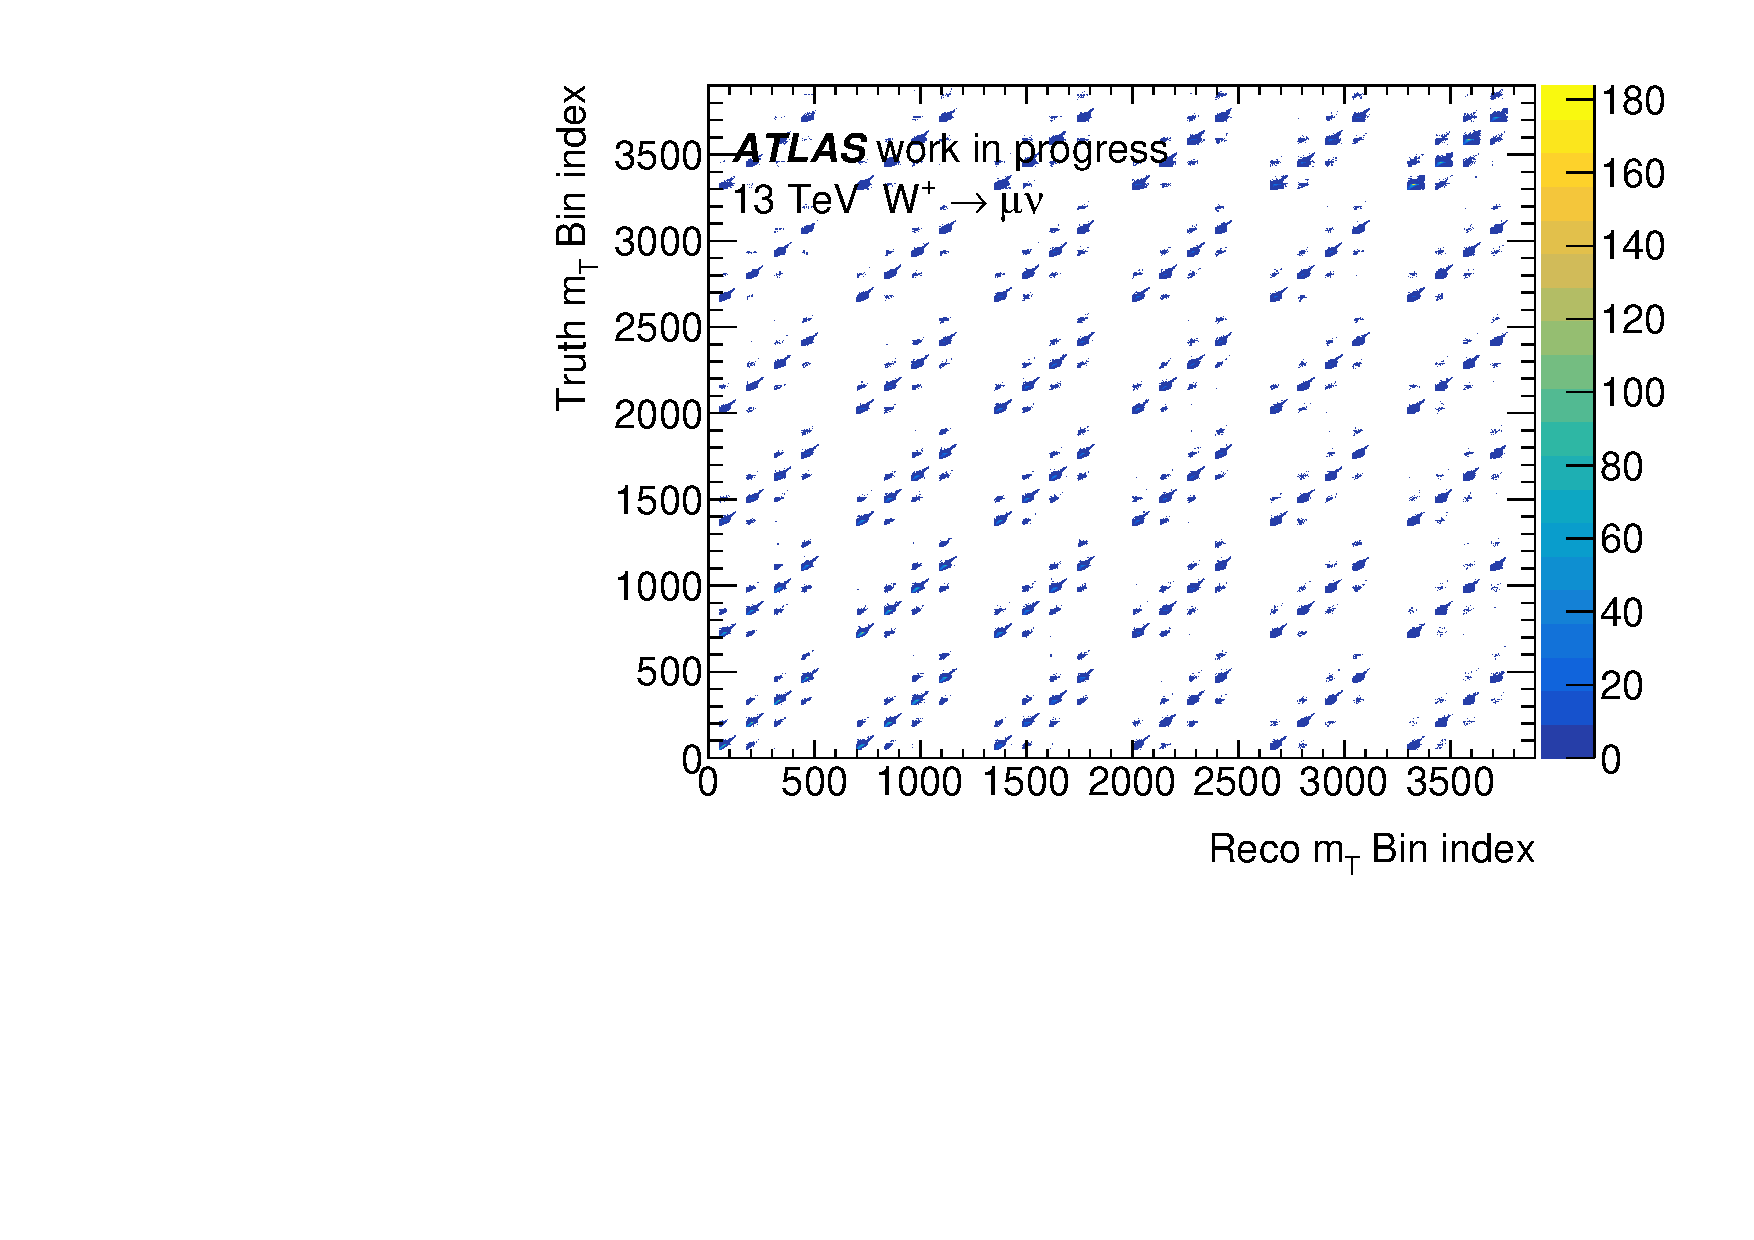
\includegraphics[width=\textwidth]{figures/electroweak/migcat_13tev_Wplusmunu_mt.pdf}
    \end{minipage}
    \hfill
    \begin{minipage}[b]{0.48\textwidth}
        \centering
        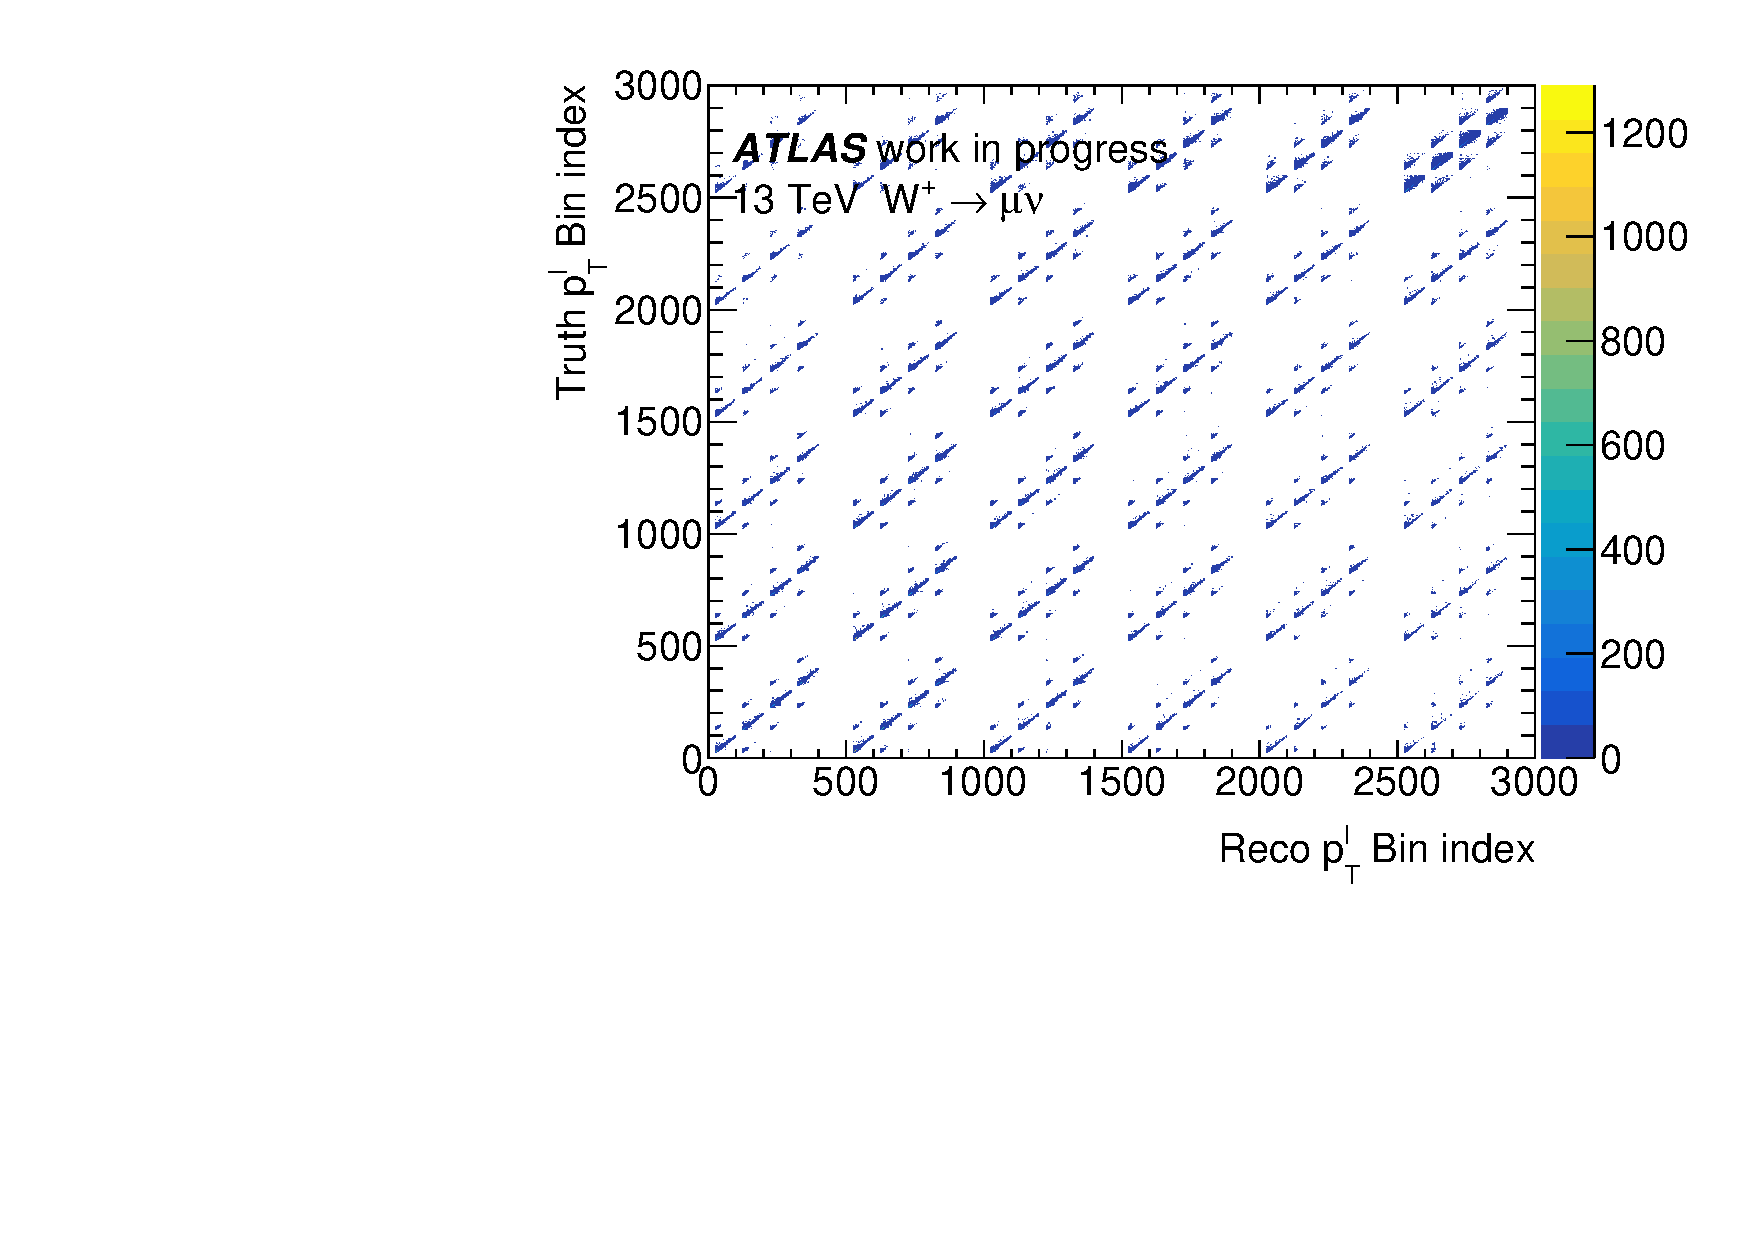
\includegraphics[width=\textwidth]{figures/electroweak/migcat_13tev_Wplusmunu_lpt.pdf}
    \end{minipage}

    \medskip
    \begin{minipage}[b]{0.48\textwidth}
        \centering
        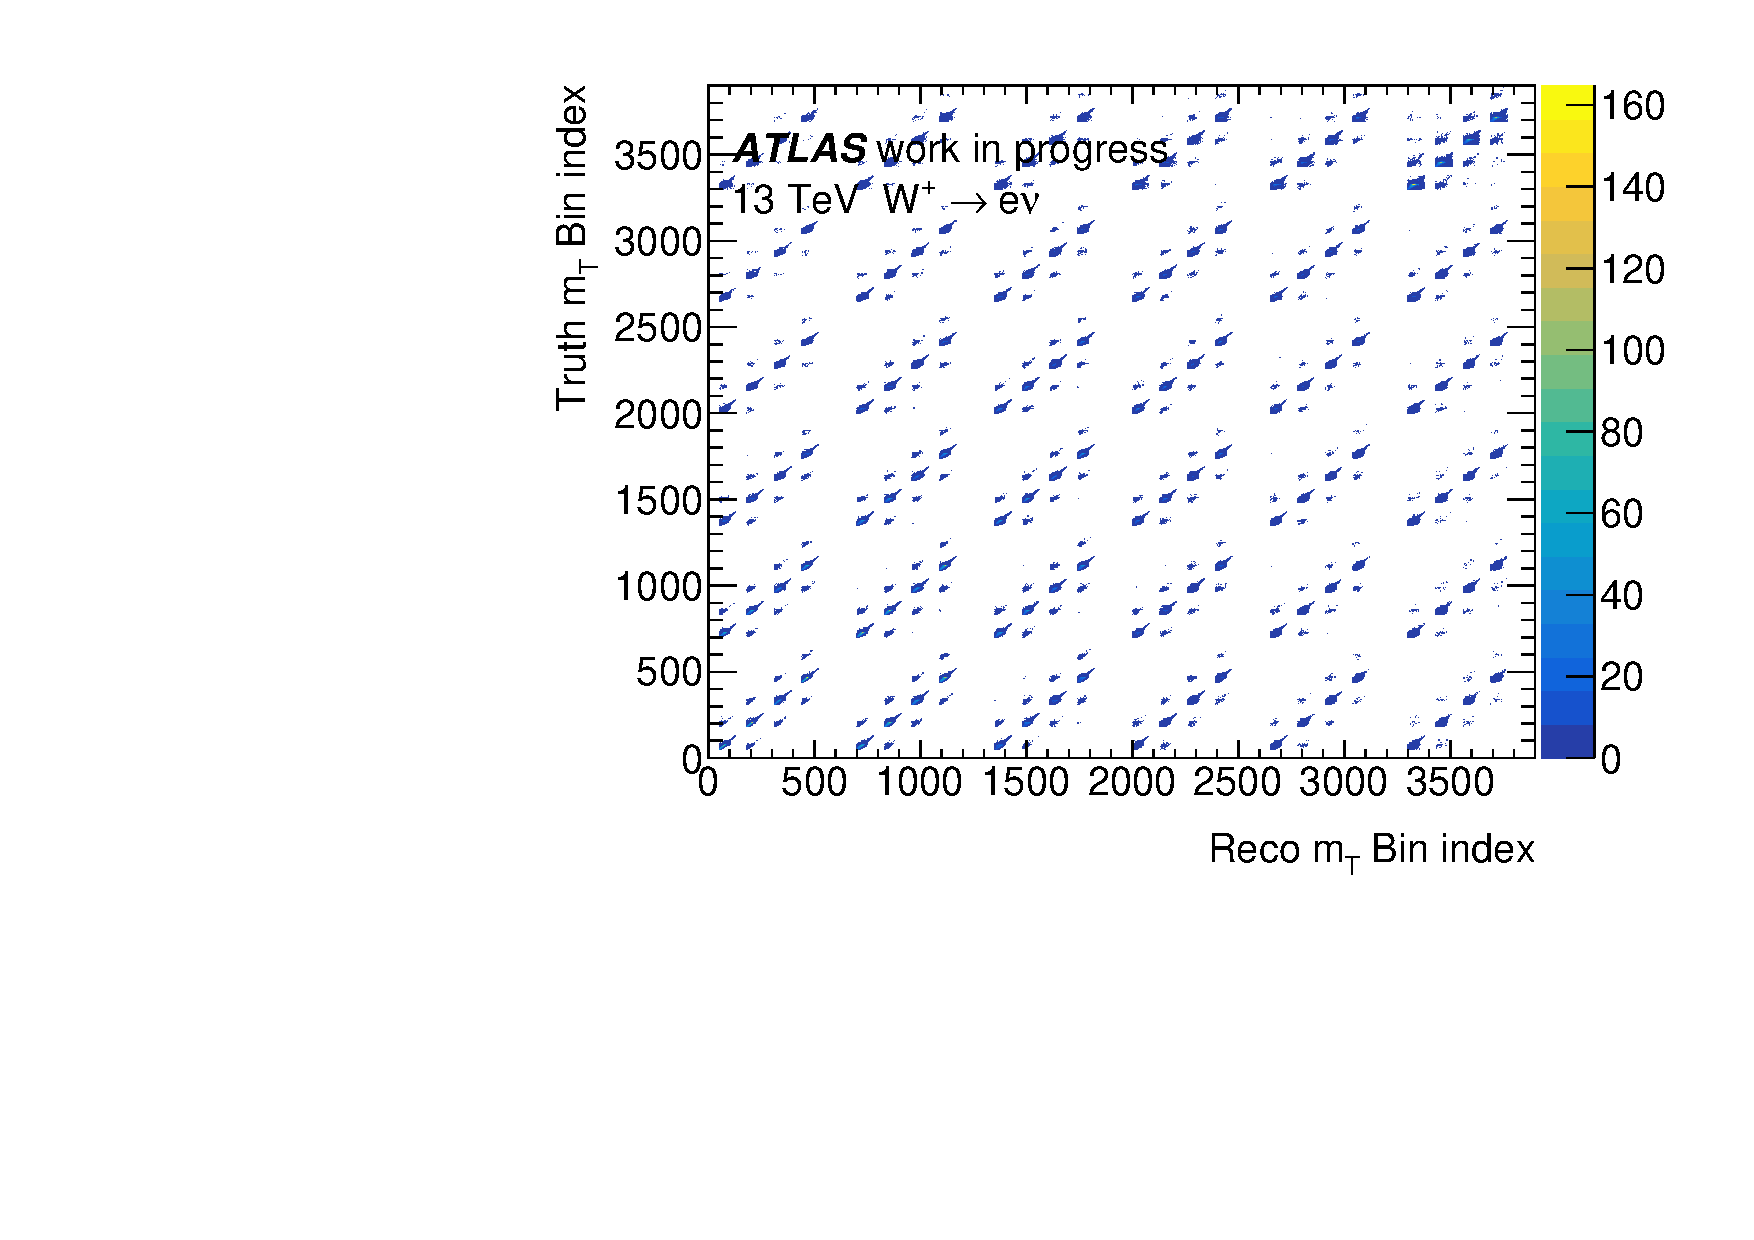
\includegraphics[width=\textwidth]{figures/electroweak/migcat_13tev_Wplusenu_mt.pdf}
    \end{minipage}
    \hfill
    \begin{minipage}[b]{0.48\textwidth}
        \centering
        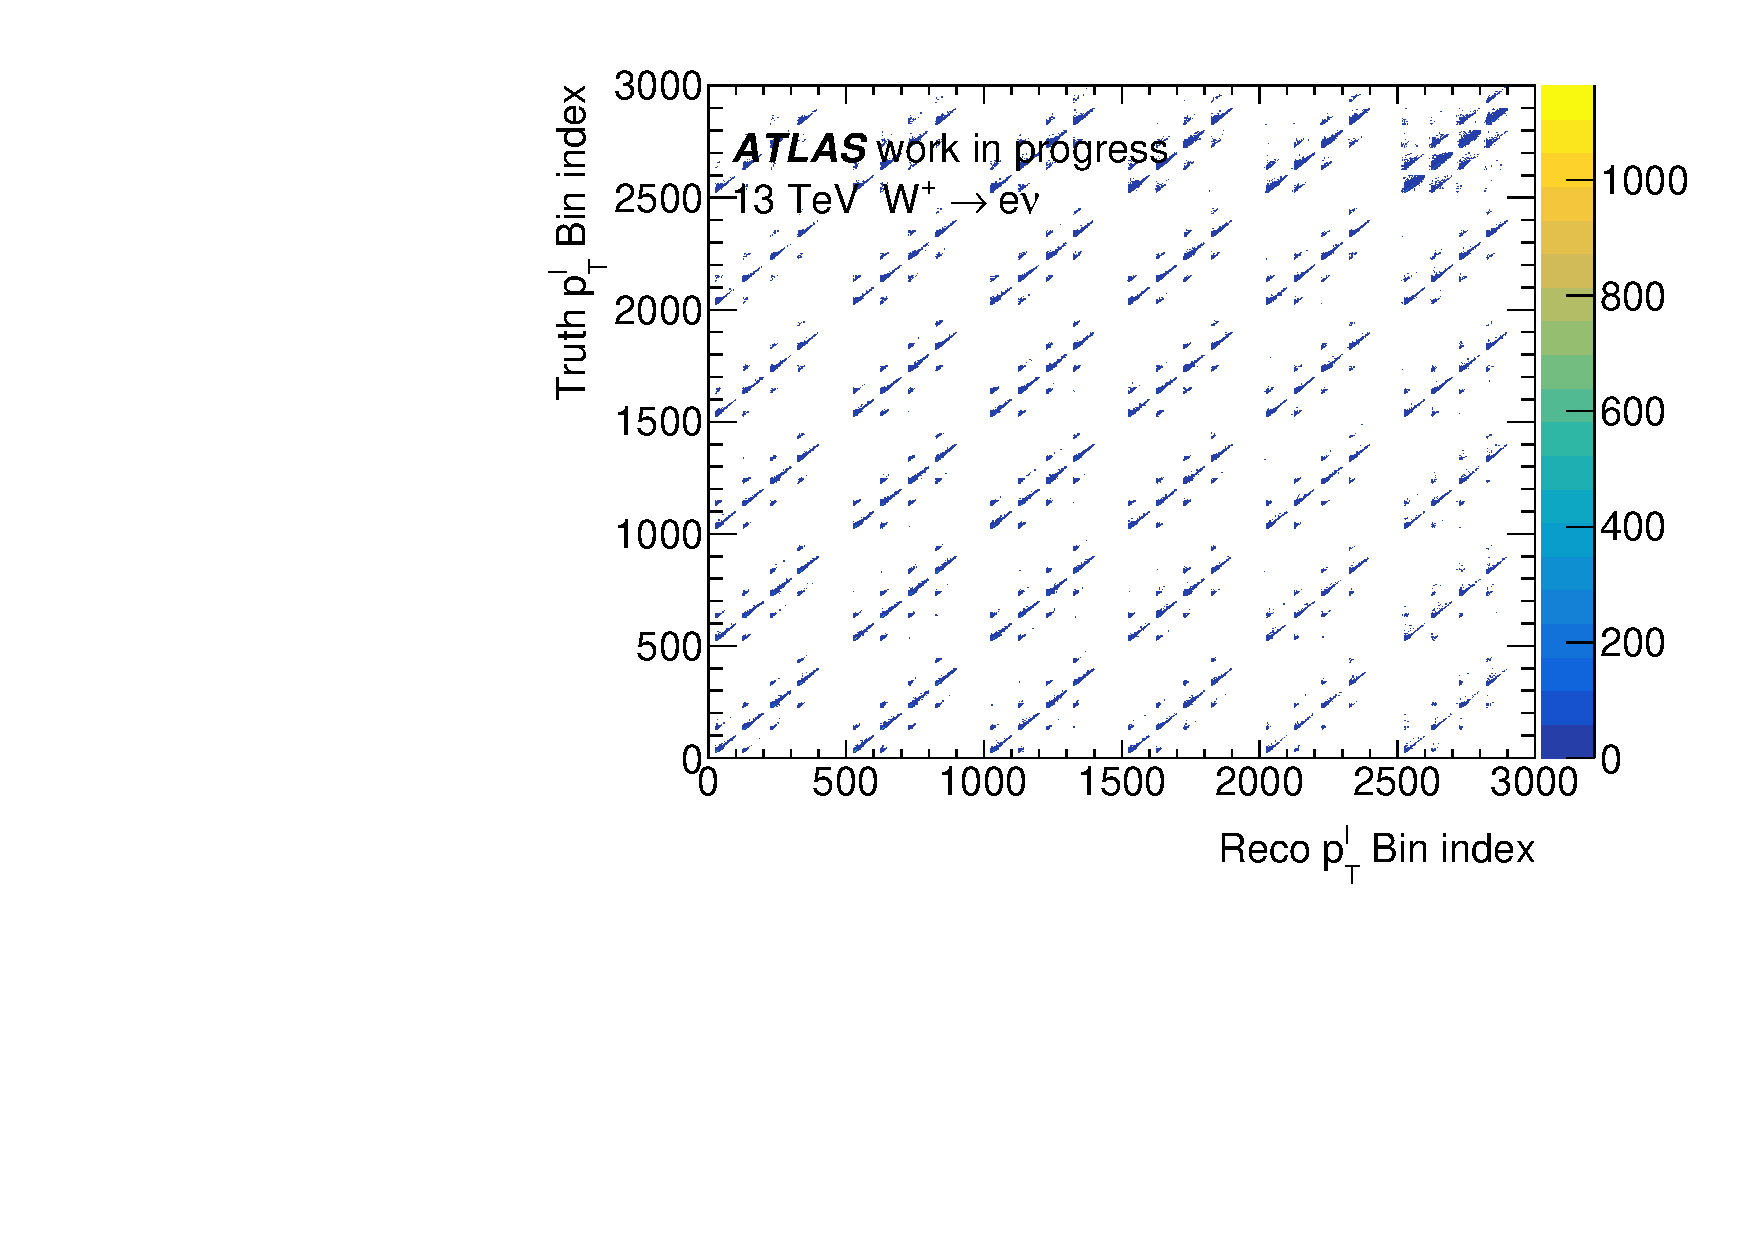
\includegraphics[width=\textwidth]{figures/electroweak/migcat_13tev_Wplusenu_lpt.pdf}
    \end{minipage}
    \caption{Unrolled migration matrix of mt(left)  and lpt (right) at 13 TeV center-of-mass energy.}
    \label{fig:migcat13}
\end{figure}

\begin{figure}[h!]
    \centering
    \begin{minipage}[b]{0.48\textwidth}
        \centering
        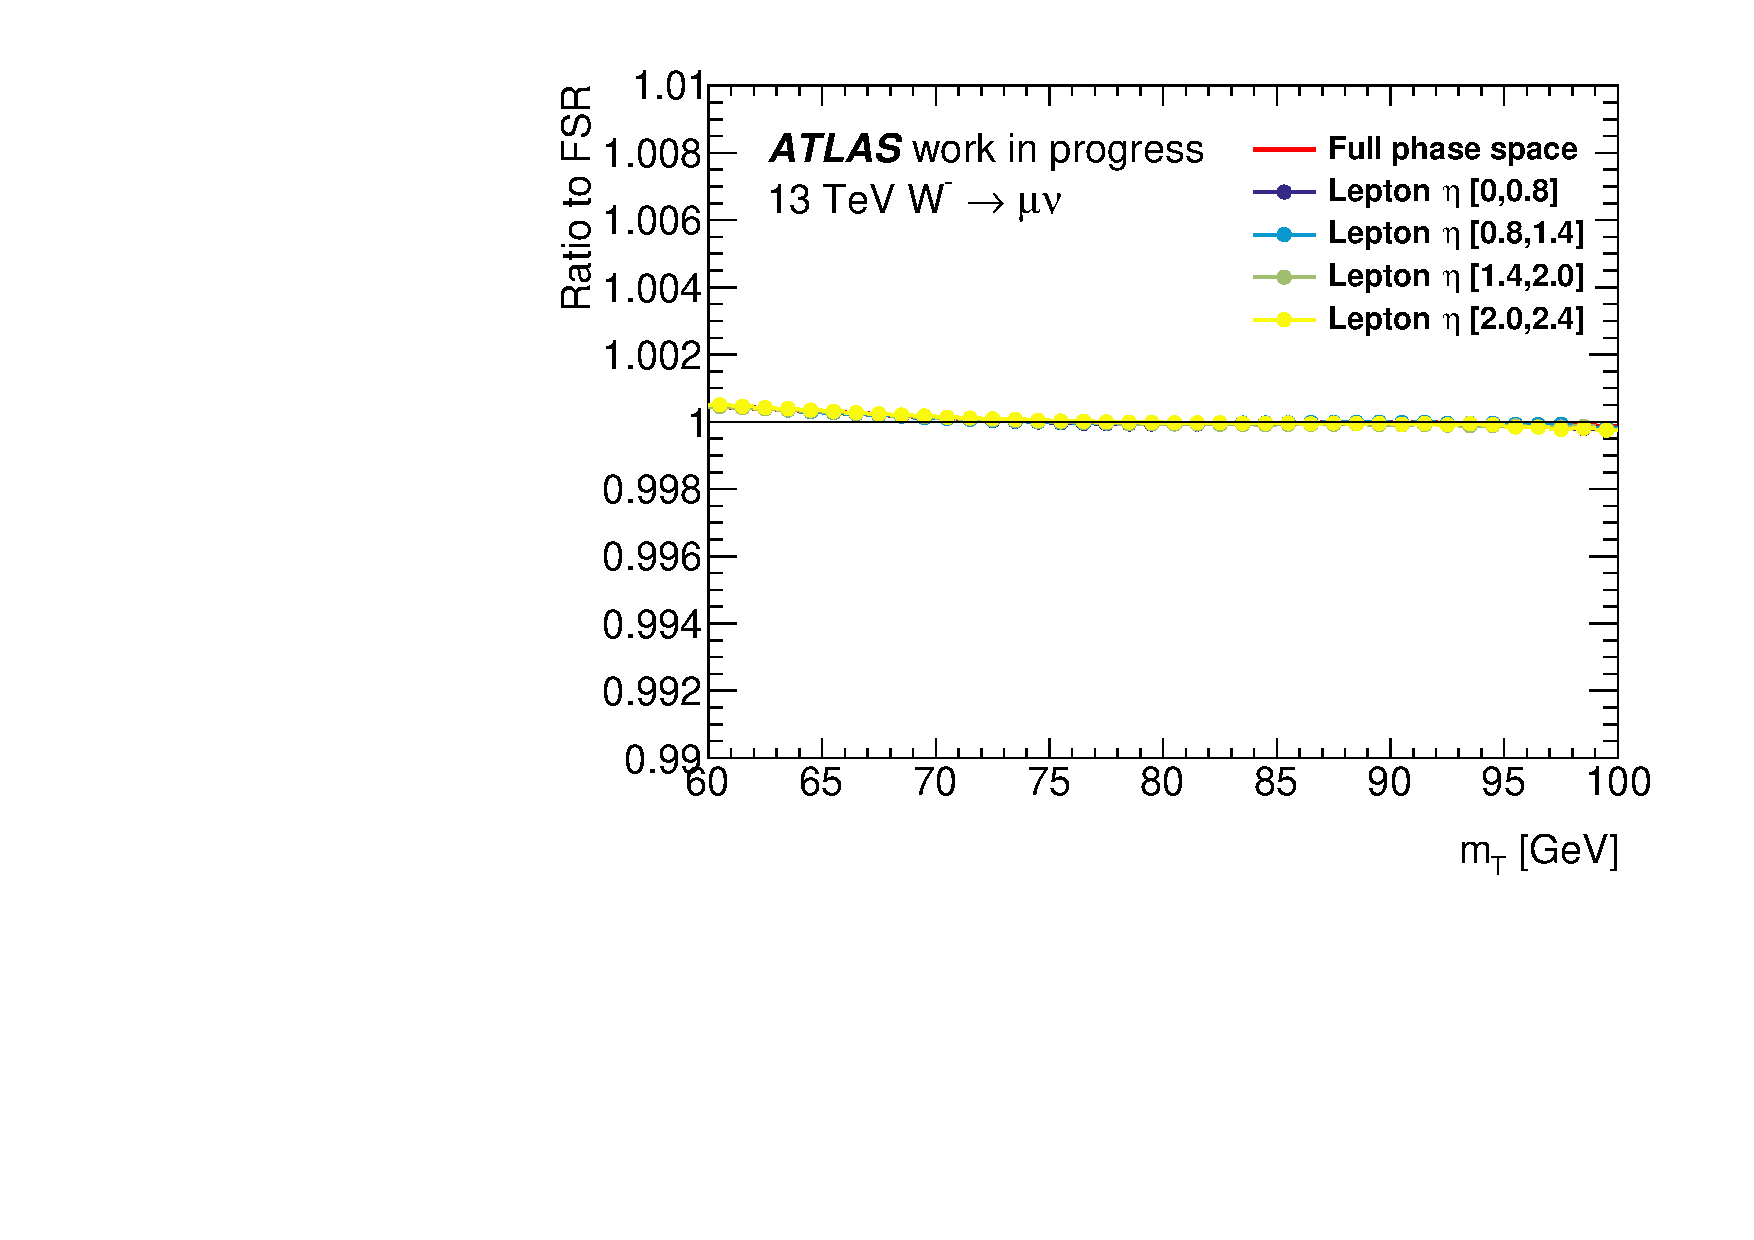
\includegraphics[width=\textwidth]{figures/electroweak/reco_letacat_13tev_wminusmuon_mt.pdf}
    \end{minipage}
    \hfill
    \begin{minipage}[b]{0.48\textwidth}
        \centering
        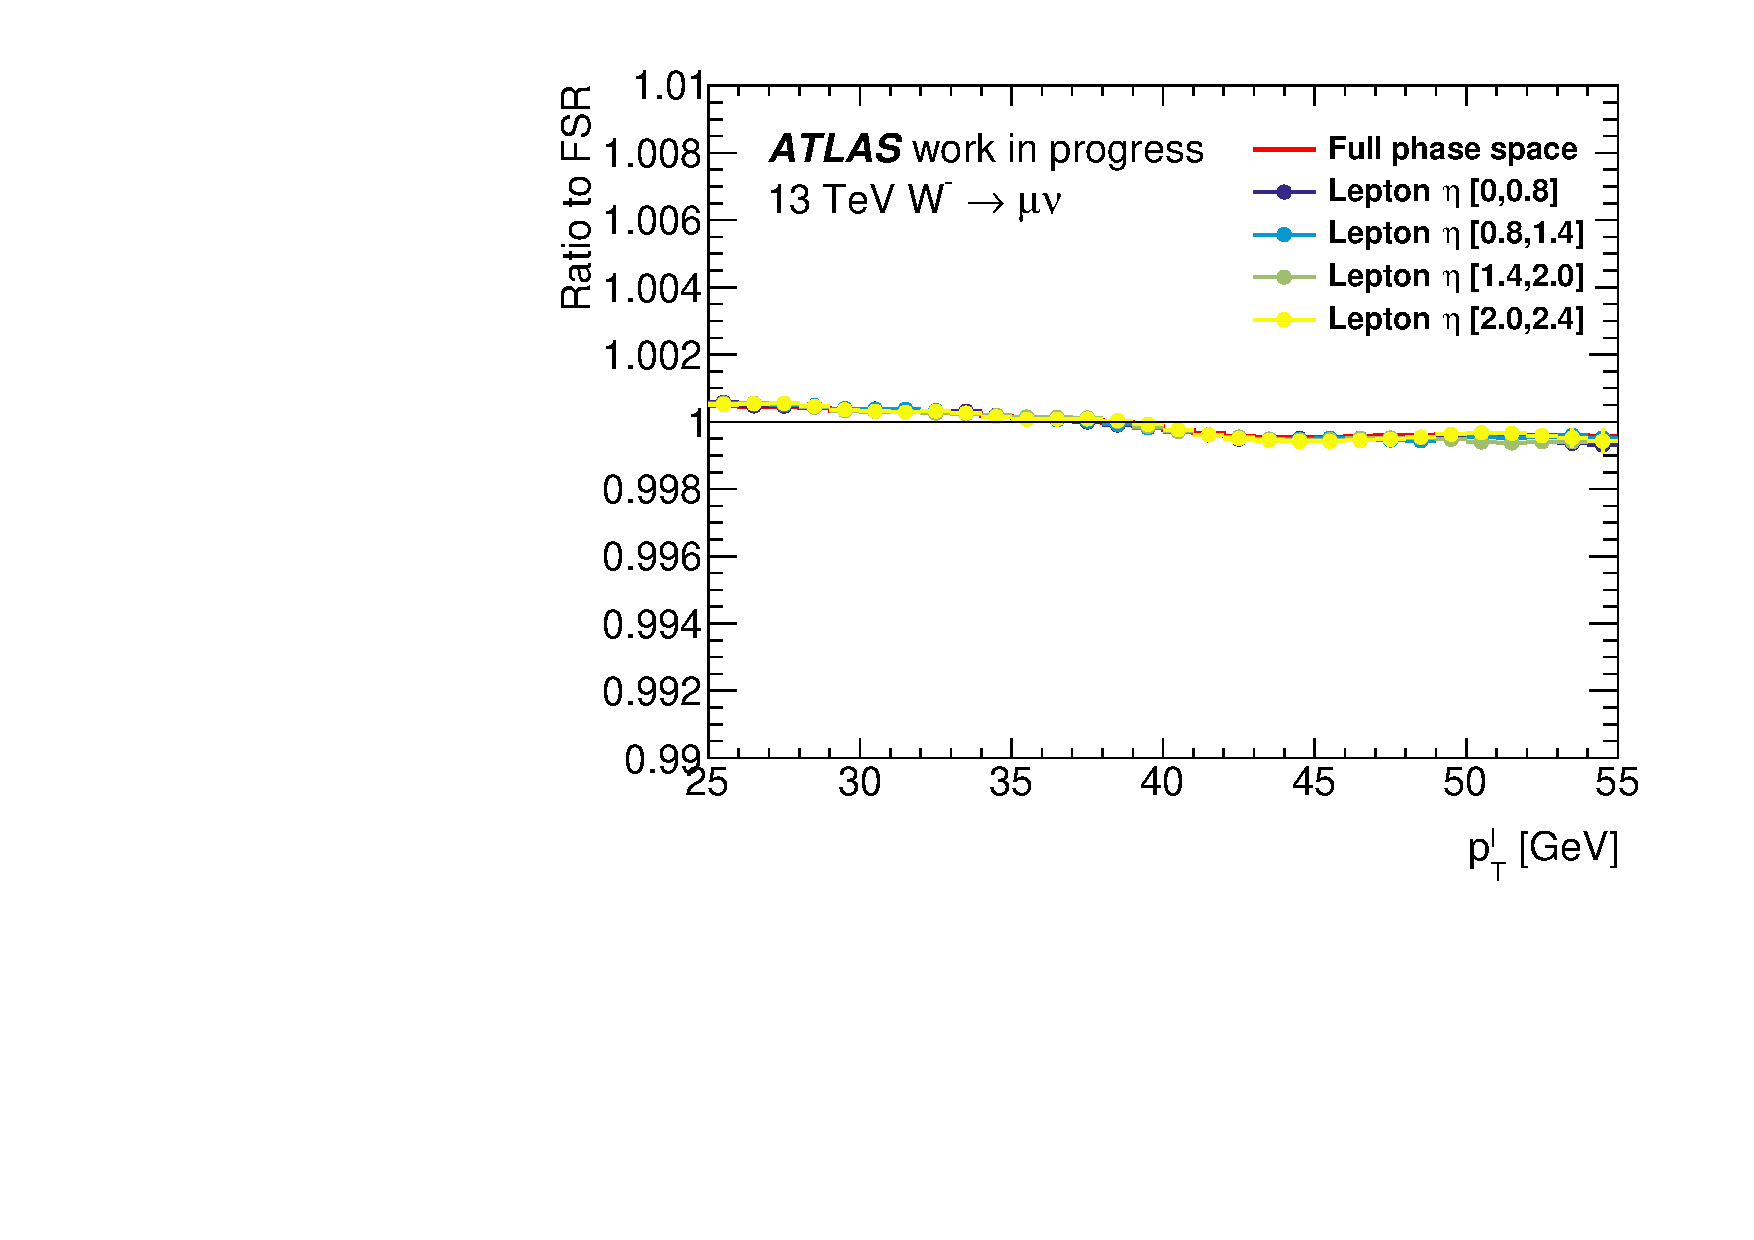
\includegraphics[width=\textwidth]{figures/electroweak/reco_letacat_13tev_wminusmuon_lpt.pdf}
    \end{minipage}

    \medskip
    \begin{minipage}[b]{0.48\textwidth}
        \centering
        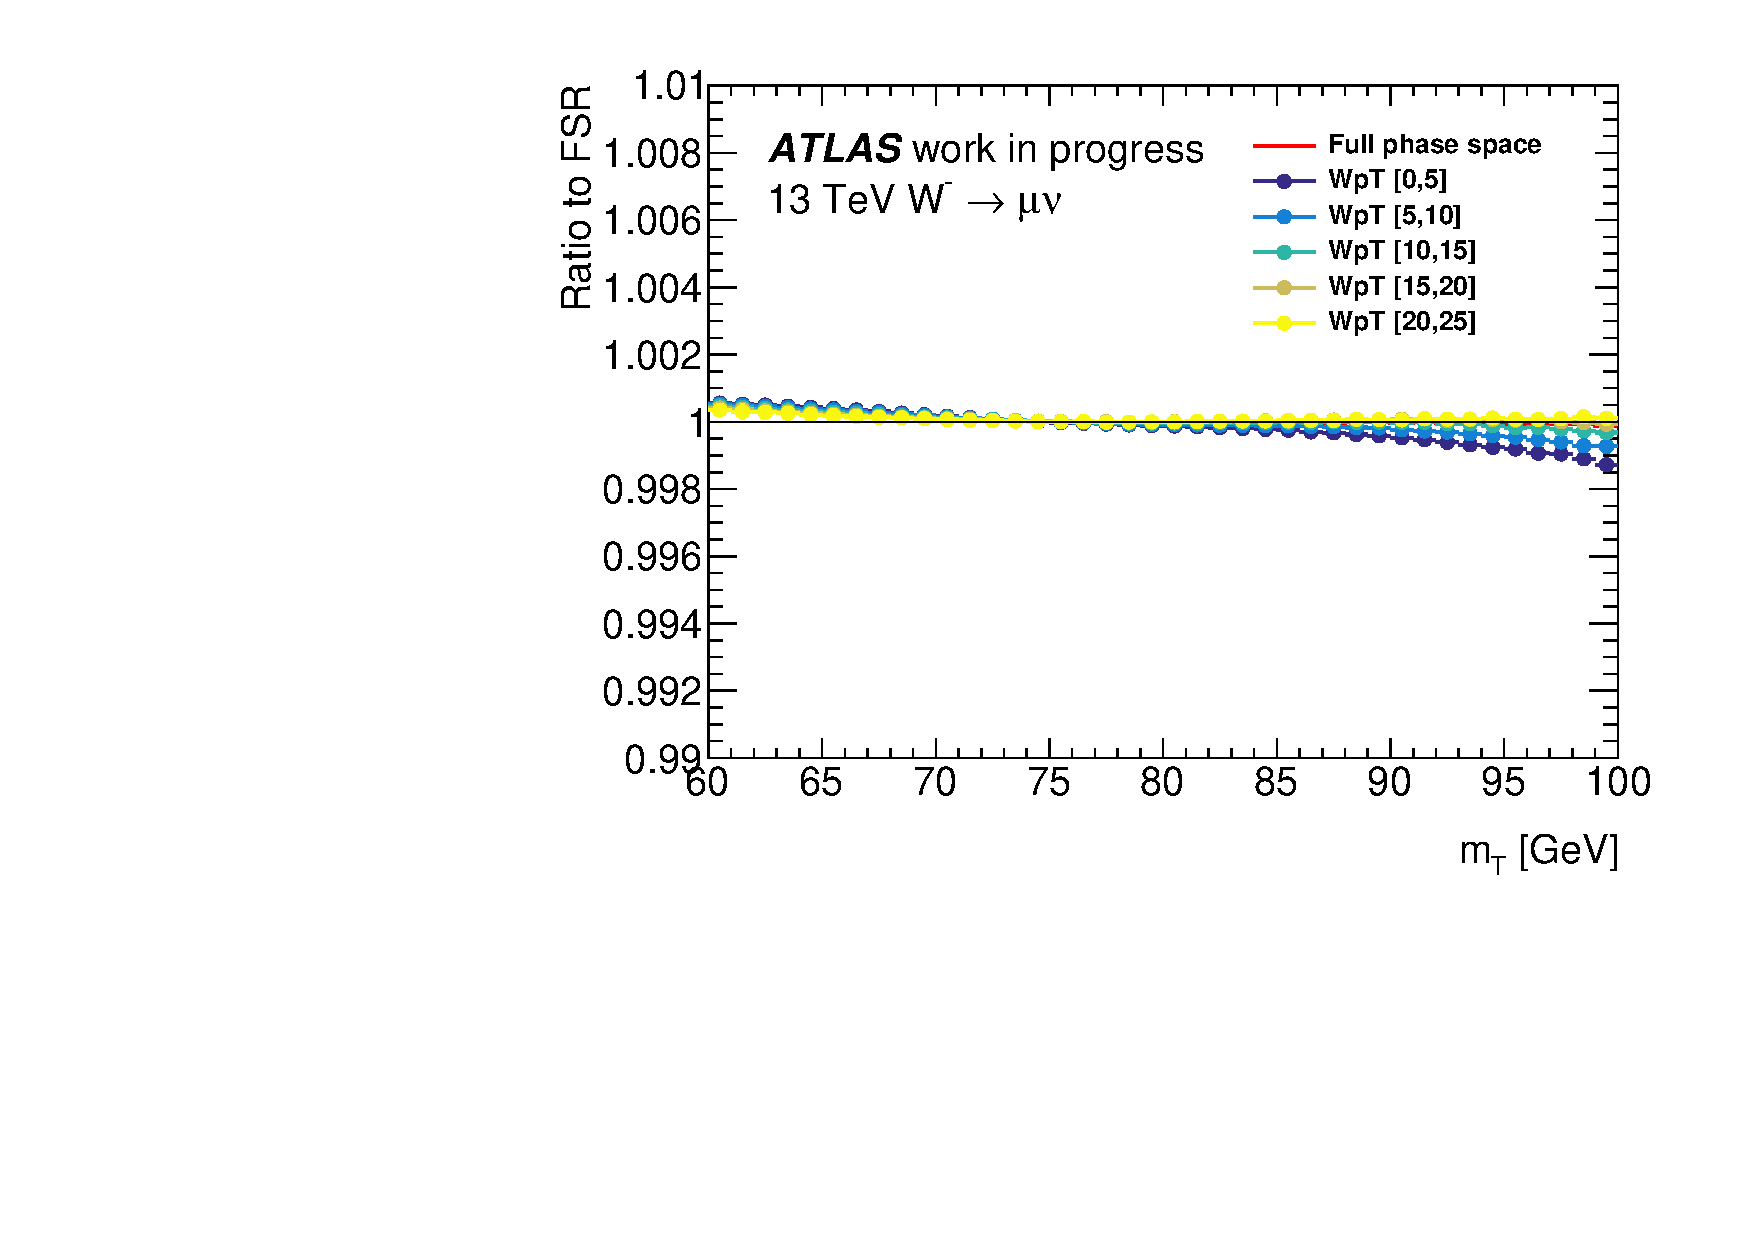
\includegraphics[width=\textwidth]{figures/electroweak/reco_wptcat_13tev_wminusmuon_mt.pdf}
    \end{minipage}
    \hfill
    \begin{minipage}[b]{0.48\textwidth}
        \centering
        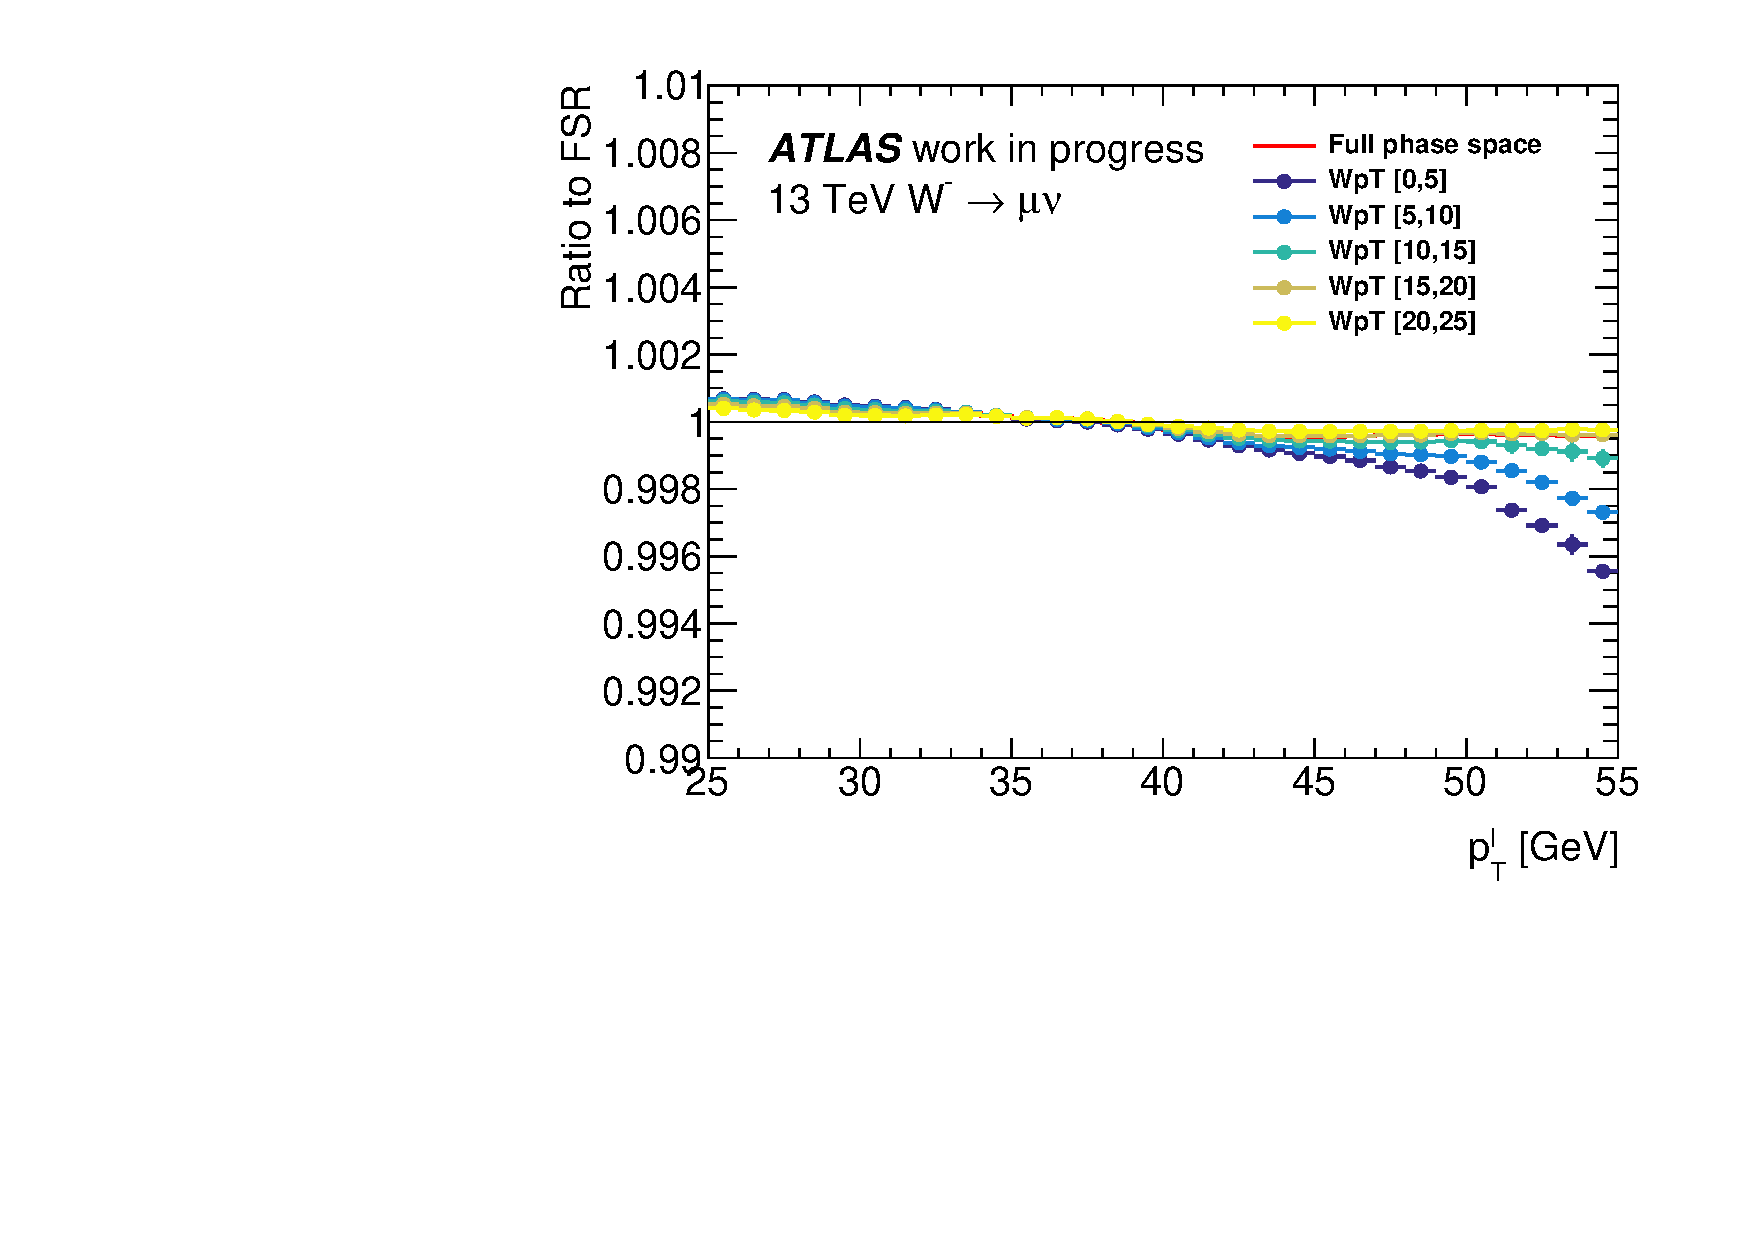
\includegraphics[width=\textwidth]{figures/electroweak/reco_wptcat_13tev_wminusmuon_lpt.pdf}
    \end{minipage}
    \caption{13 TeV $W^+\rightarrow\mu\nu$ channel high order EW corrections on each category of mt (left) and lpt (right) at different  $|\eta_l|$ (top) and ptw\ (bottom) values compared with full phase correction at detector level.}
    \label{fig:13wpm_wptleta_reco}
\end{figure}
